\subsection{Overview}
    \begin{frame}
        \frametitle{Overview}
        In this defense, I will show that I successfully: 
        \pause
        \begin{enumerate}
            \item Furthered our understanding of the \gls{AHTR} design's complexities 
            through neutronics and temperature modeling
            \pause
            \item Created an open-source tool that enables reactor generative 
            design optimization with evolutionary algorithms
            \pause
            \item Applied the optimization tool to the \gls{AHTR} design for 
            non-conventional geometries and fuel distributions 
        \end{enumerate}
    \end{frame}

\subsection{Background: Advanced High Temperature Reactor}
    \begin{frame}
        \frametitle{MSR + VHTR = FHR}
        Gen IV Forum identified \textbf{new and innovative Gen IV nuclear energy systems}: 
        Molten Salt Reactors (MSR) and Very High-Temperature Reactors (VHTR). 
        \pause
        \vspace{0.2cm}
        \begin{columns}
        \begin{column}{0.5\textwidth}
        The \textbf{Fluoride-Salt Cooled High-Temperature Reactor (FHR) concept 
        combines the best aspects of MSR and VHTR}.

        The \acrfull{AHTR} is a subset of the FHR. 
        \vspace{-0.6cm}
        \begin{figure}[]
            \makebox[\textwidth][c]{
                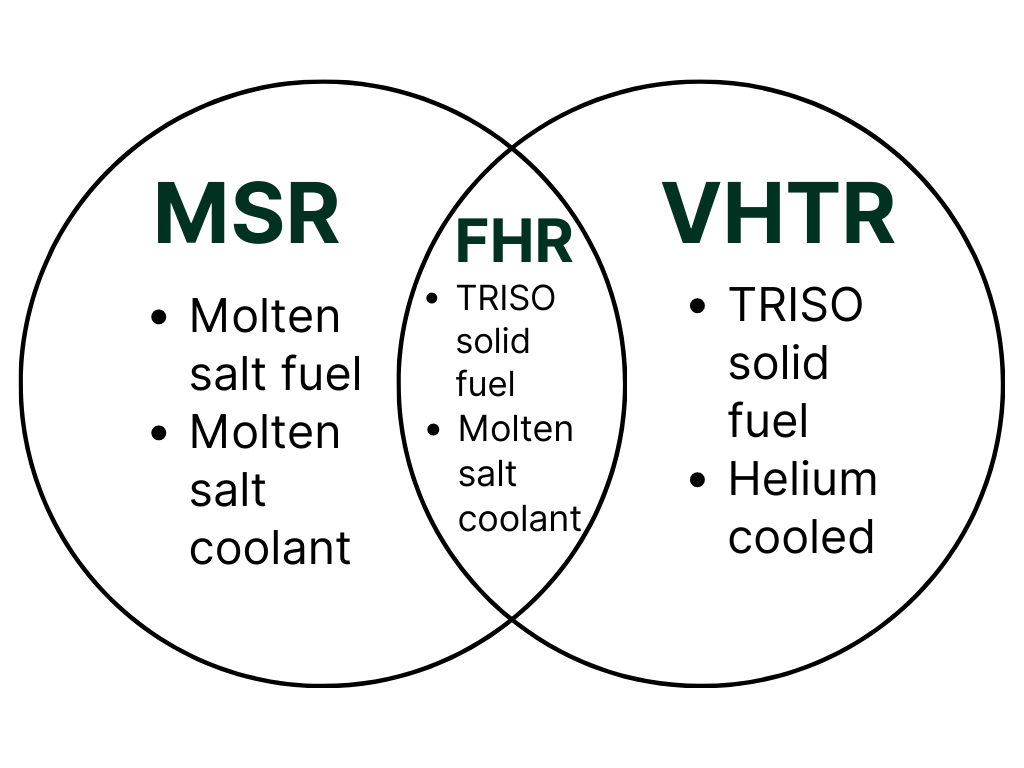
\includegraphics[width=1.05\linewidth]{figures/fhr_venn.png}} 
            %\caption{FHR Venn diagram.}
        \end{figure}
        \end{column}
        \pause
        \begin{column}{0.5\textwidth}
            \acrfull{FLiBe} salt cooled: \textbf{superior cooling, low operating 
            pressure}. 
            
            \vspace{0.2cm}
            \acrfull{TRISO} fuel: fuel kernel encapsulated in three other layers, 
            \textbf{extra barriers to fission product release, higher safety margin}. 
            \vspace{-0.1cm}
            \begin{figure}[htbp!]
                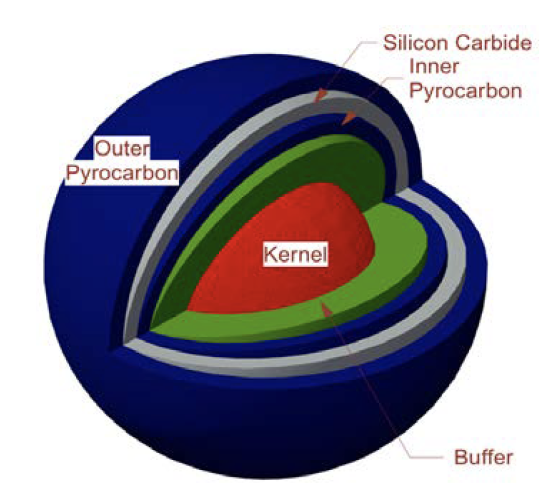
\includegraphics[width=0.45\linewidth]{../docs/figures/ahtr-triso.png}
                \caption{Tristructural Isotropic (TRISO) 
                particle. Diameter $\approx 8mm$.}
            \end{figure}
        \end{column}
    \end{columns}
        \end{frame}

    \begin{frame}
    \frametitle{Advanced High Temperature Reactor Design}
        \begin{itemize}
        \item Design developed by Oak Ridge National Laboratory
        \item Prismatic FHR design with 252 hexagonal fuel assemblies consisting of 
        18 fuel planks arranged in 3 diamond-shaped sectors
        \end{itemize}
    
    \vspace{0.2cm}
    \begin{figure}[]
        \centering
        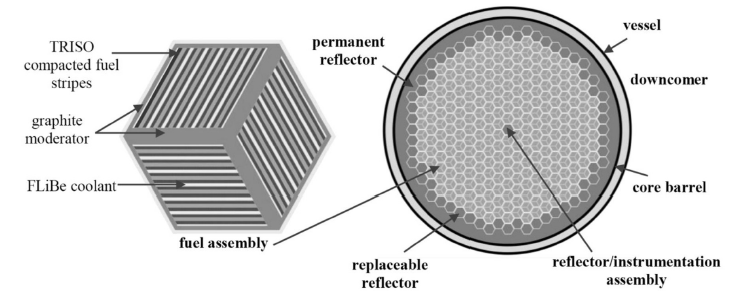
\includegraphics[width=\linewidth]{../docs/figures/ahtr.png} 
        \caption{\acrlong{AHTR} fuel assembly (left) and core configuration (right) 
        reproduced from \cite{ramey_monte_2018}.}
        \label{fig:ahtr}
    \end{figure}
    \end{frame}

    \begin{frame}
    \frametitle{Advanced High Temperature Reactor Geometry}
    \begin{figure}[]
        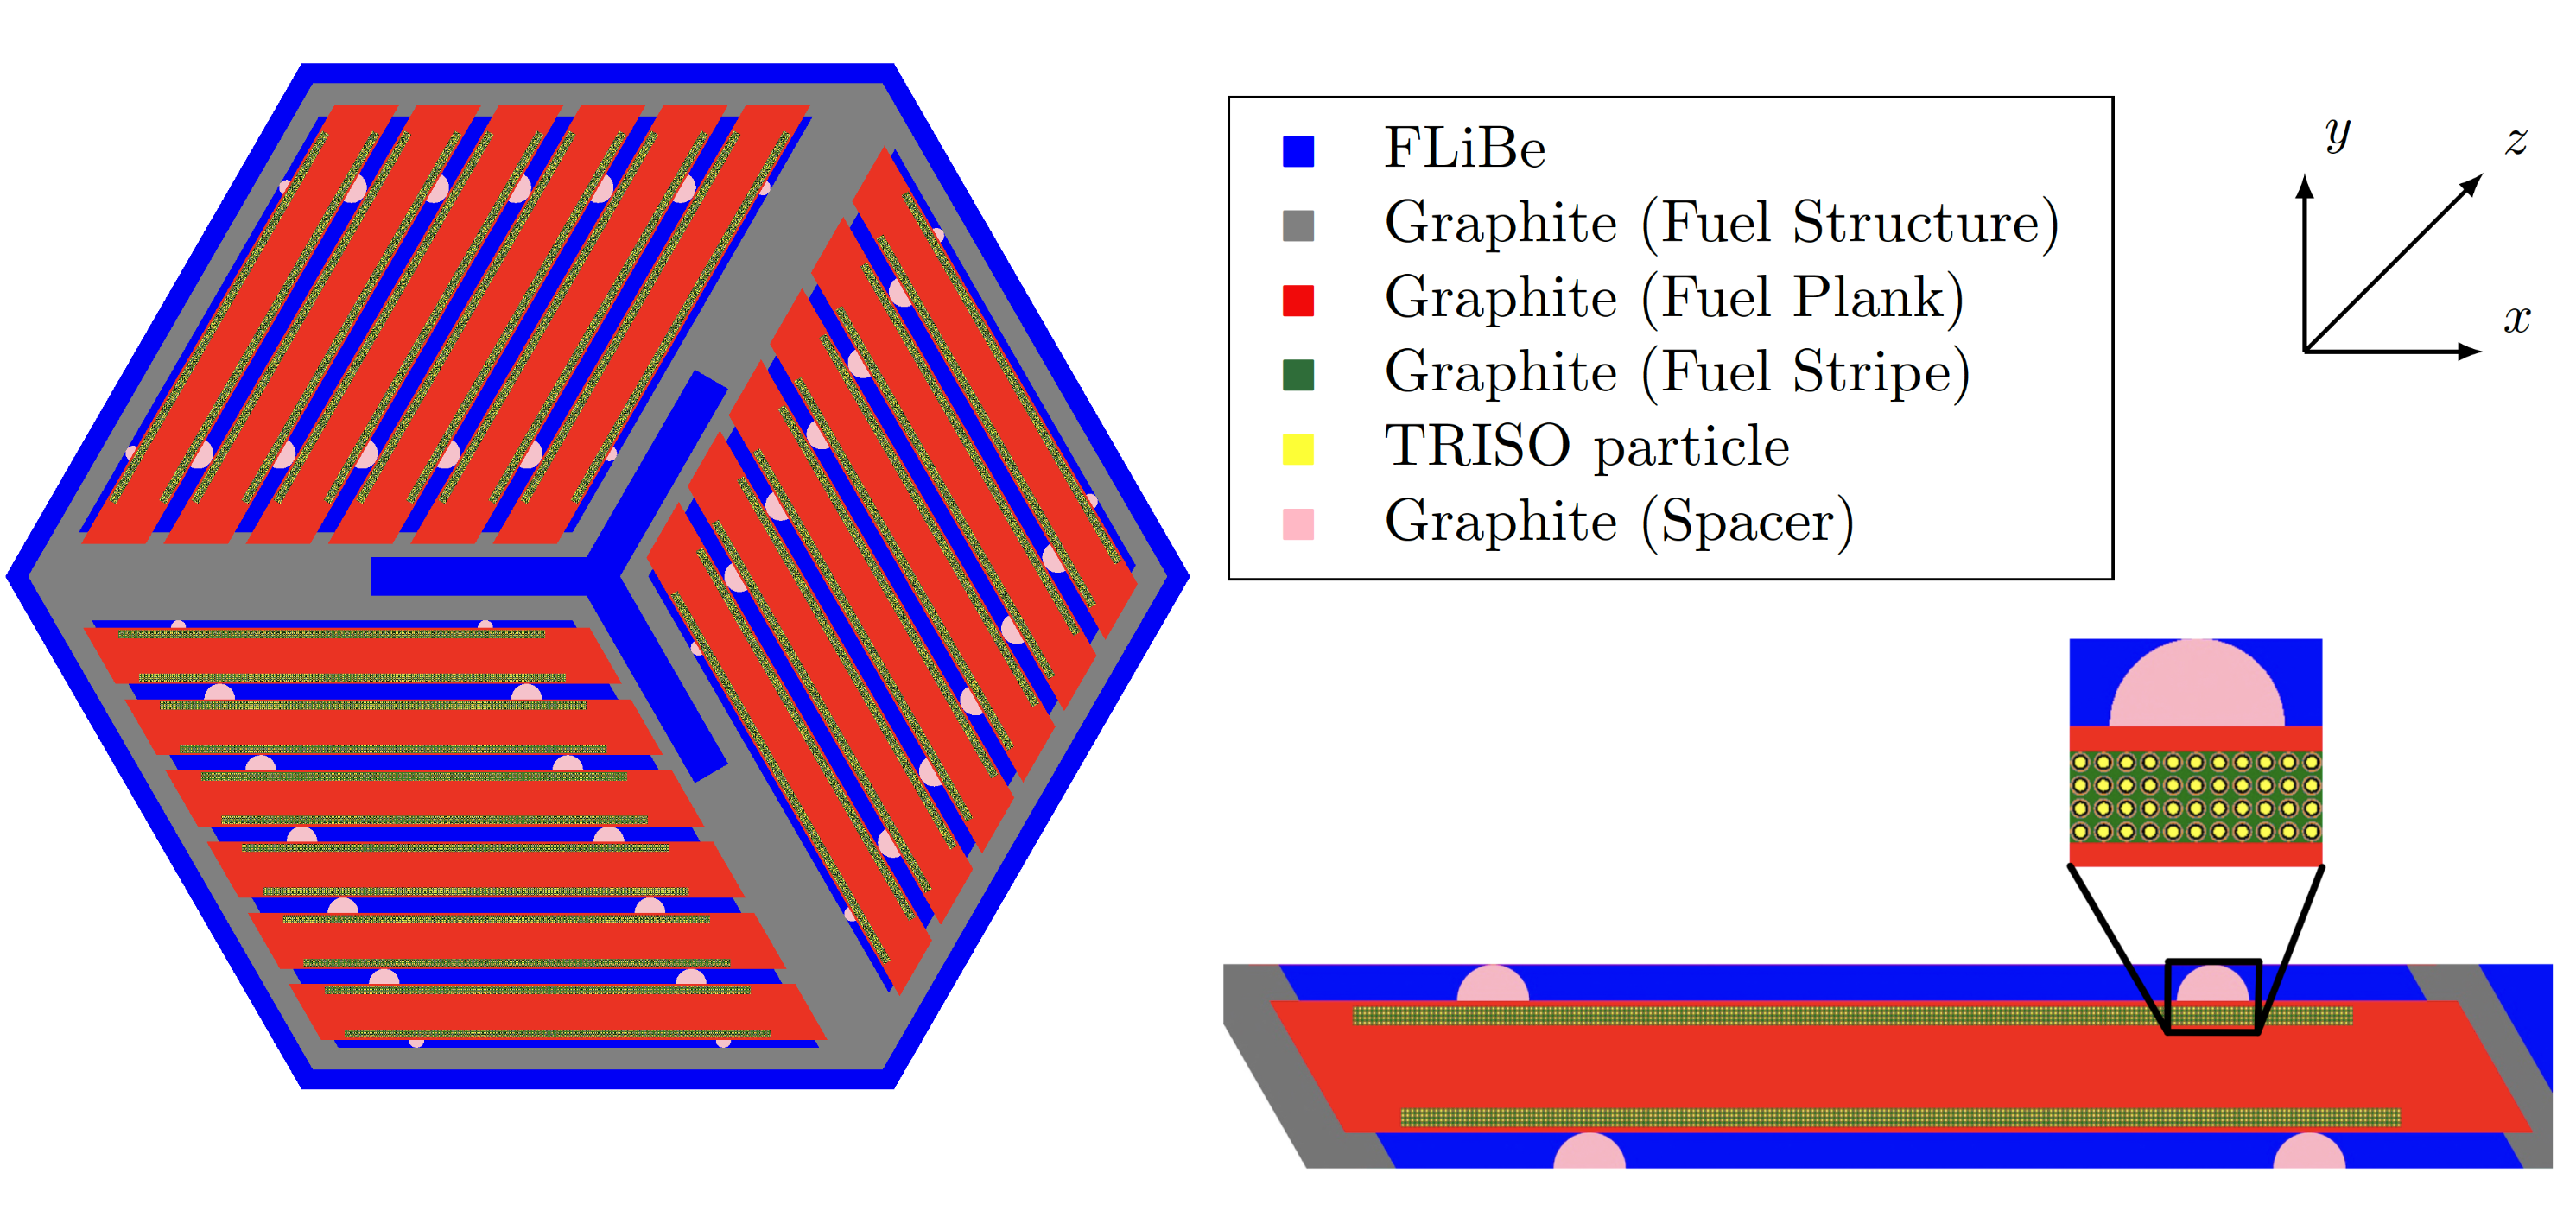
\includegraphics[width=\linewidth]{figures/ahtr-assembly.png} 
        \caption{AHTR fuel assembly with 18 fuel plates arranged in 
        three diamond-shaped sectors, with a central Y-shaped and external channel 
        graphite structure.}
    \end{figure}
    \pause
    \vspace{-0.2cm}
    The AHTR fuel has \textbf{triple heterogeneity}: hexagonal fuel elements within the 
    core, and TRISO particles embedded in stripes within each plank.
    \end{frame}

    \begin{frame}
    \frametitle{FHR Benchmark}
    The AHTR's geometry's triple heterogeneity results in
    \textbf{complex reactor physics} and \textbf{significant modeling challenges}.
    \begin{itemize}
        \item Many surfaces to model = computationally expensive 
        \item Homogenization might result in loss of reactor physics effects 
    \end{itemize}
    \pause
    \vspace{0.3cm}
    In 2019 the \textbf{OECD-NEA initiated the FHR benchmark}. Its objective 
    is to identify the applicability, accuracy, and practicality of the latest 
    methods and codes to assess the current state of the art for FHR modeling.

    \vspace{0.2cm}
    \begin{figure}[]
        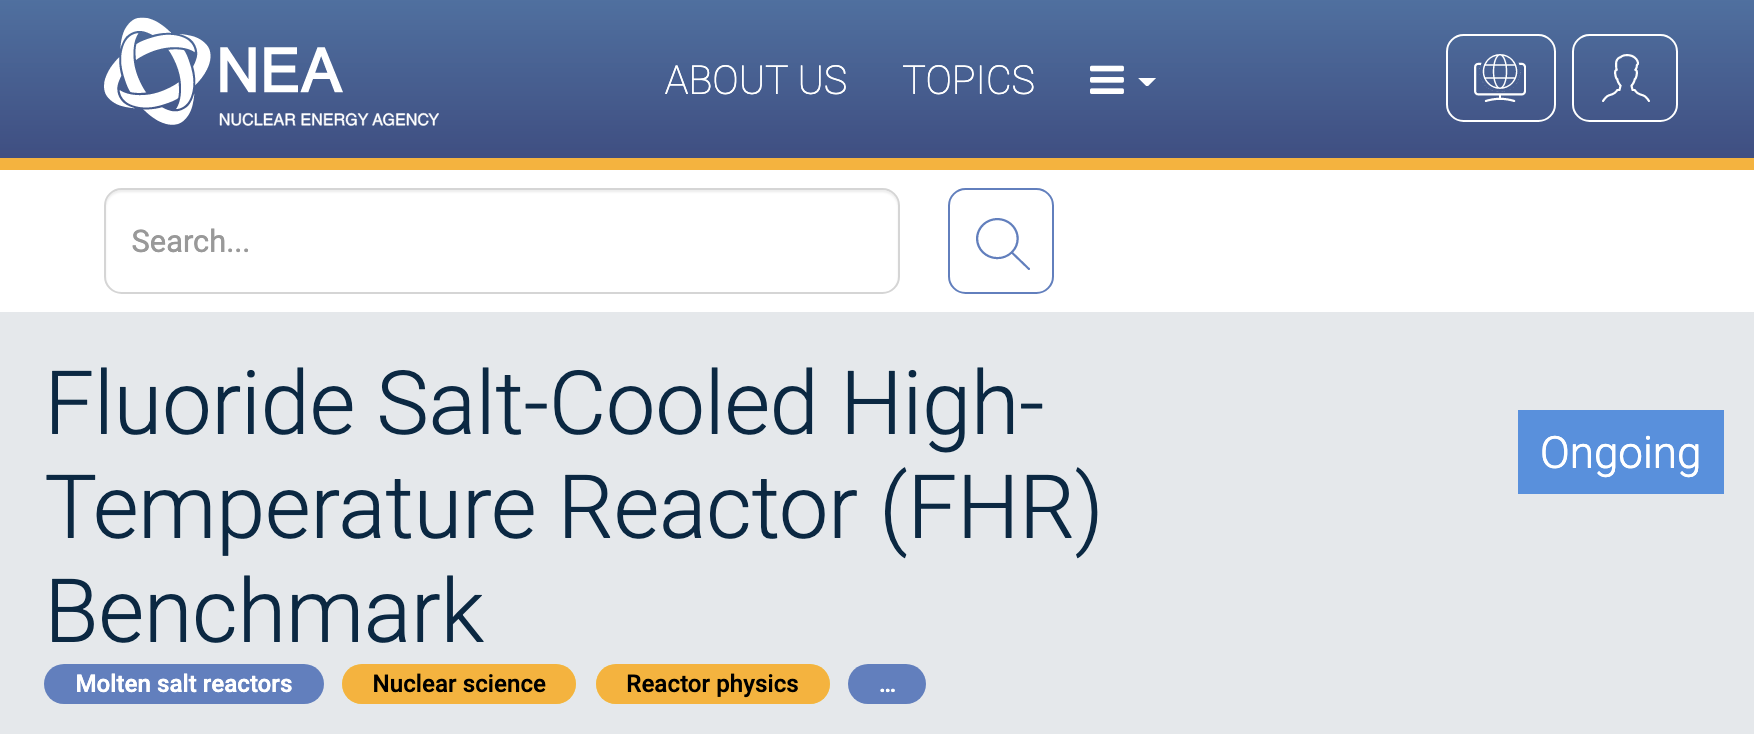
\includegraphics[width=0.7\linewidth]{figures/benchmark.png} 
        \caption{OECD NEA's FHR Benchmark \cite{petrovic_benchmark_2021}.}
    \end{figure}
    \end{frame}

\subsection{Objectives: AHTR Model Development}
    \begin{frame}
        \frametitle{Research Objectives: AHTR Model Development}
        \begin{block}{Technical Gap}
            The geometrically complex AHTR design is challenging to model accurately 
            and computationally expensive. 
        \end{block}
        \pause
        \begin{block}{Research Objectives: AHTR Model Development}
        \begin{itemize}
            \item Participate in FHR benchmark's neutronics modeling to further our 
            understanding of the AHTR design's complexities
            \item AHTR temperature model to capture thermal feedback effects
        \end{itemize}
        \end{block}
        \pause
        \begin{block}{Link to Reactor Optimization for Non-conventional Designs}
        \begin{itemize}
        \item By participating in the benchmark, I ensure an accurate AHTR base model
        \item Thus, I can expect accurate answers for the optimized AHTR designs
        \end{itemize}
        \end{block}
    \end{frame}

\subsection{Background: Generative Reactor Design Optimization}
\begin{frame}
    \frametitle{Overview}
    In this defense, I will show that I successfully: 
    \begin{enumerate}
        \item Furthered our understanding of the \gls{AHTR} design's complexities 
        through neutronics and temperature modeling
        \item Created an open-source tool that enables reactor generative 
        design optimization with evolutionary algorithms
        \item Applied the optimization tool to the \gls{AHTR} design for 
        non-conventional geometries and fuel distributions 
    \end{enumerate}
\end{frame}

\begin{frame}
    \frametitle{3D Printing a Nuclear Reactor}
    Additive manufacturing enables us to \textbf{surpass classical 
    manufacturing constraints} and optimize for \textbf{arbitrary geometries and 
    parameters}. 
    \begin{figure}[]
        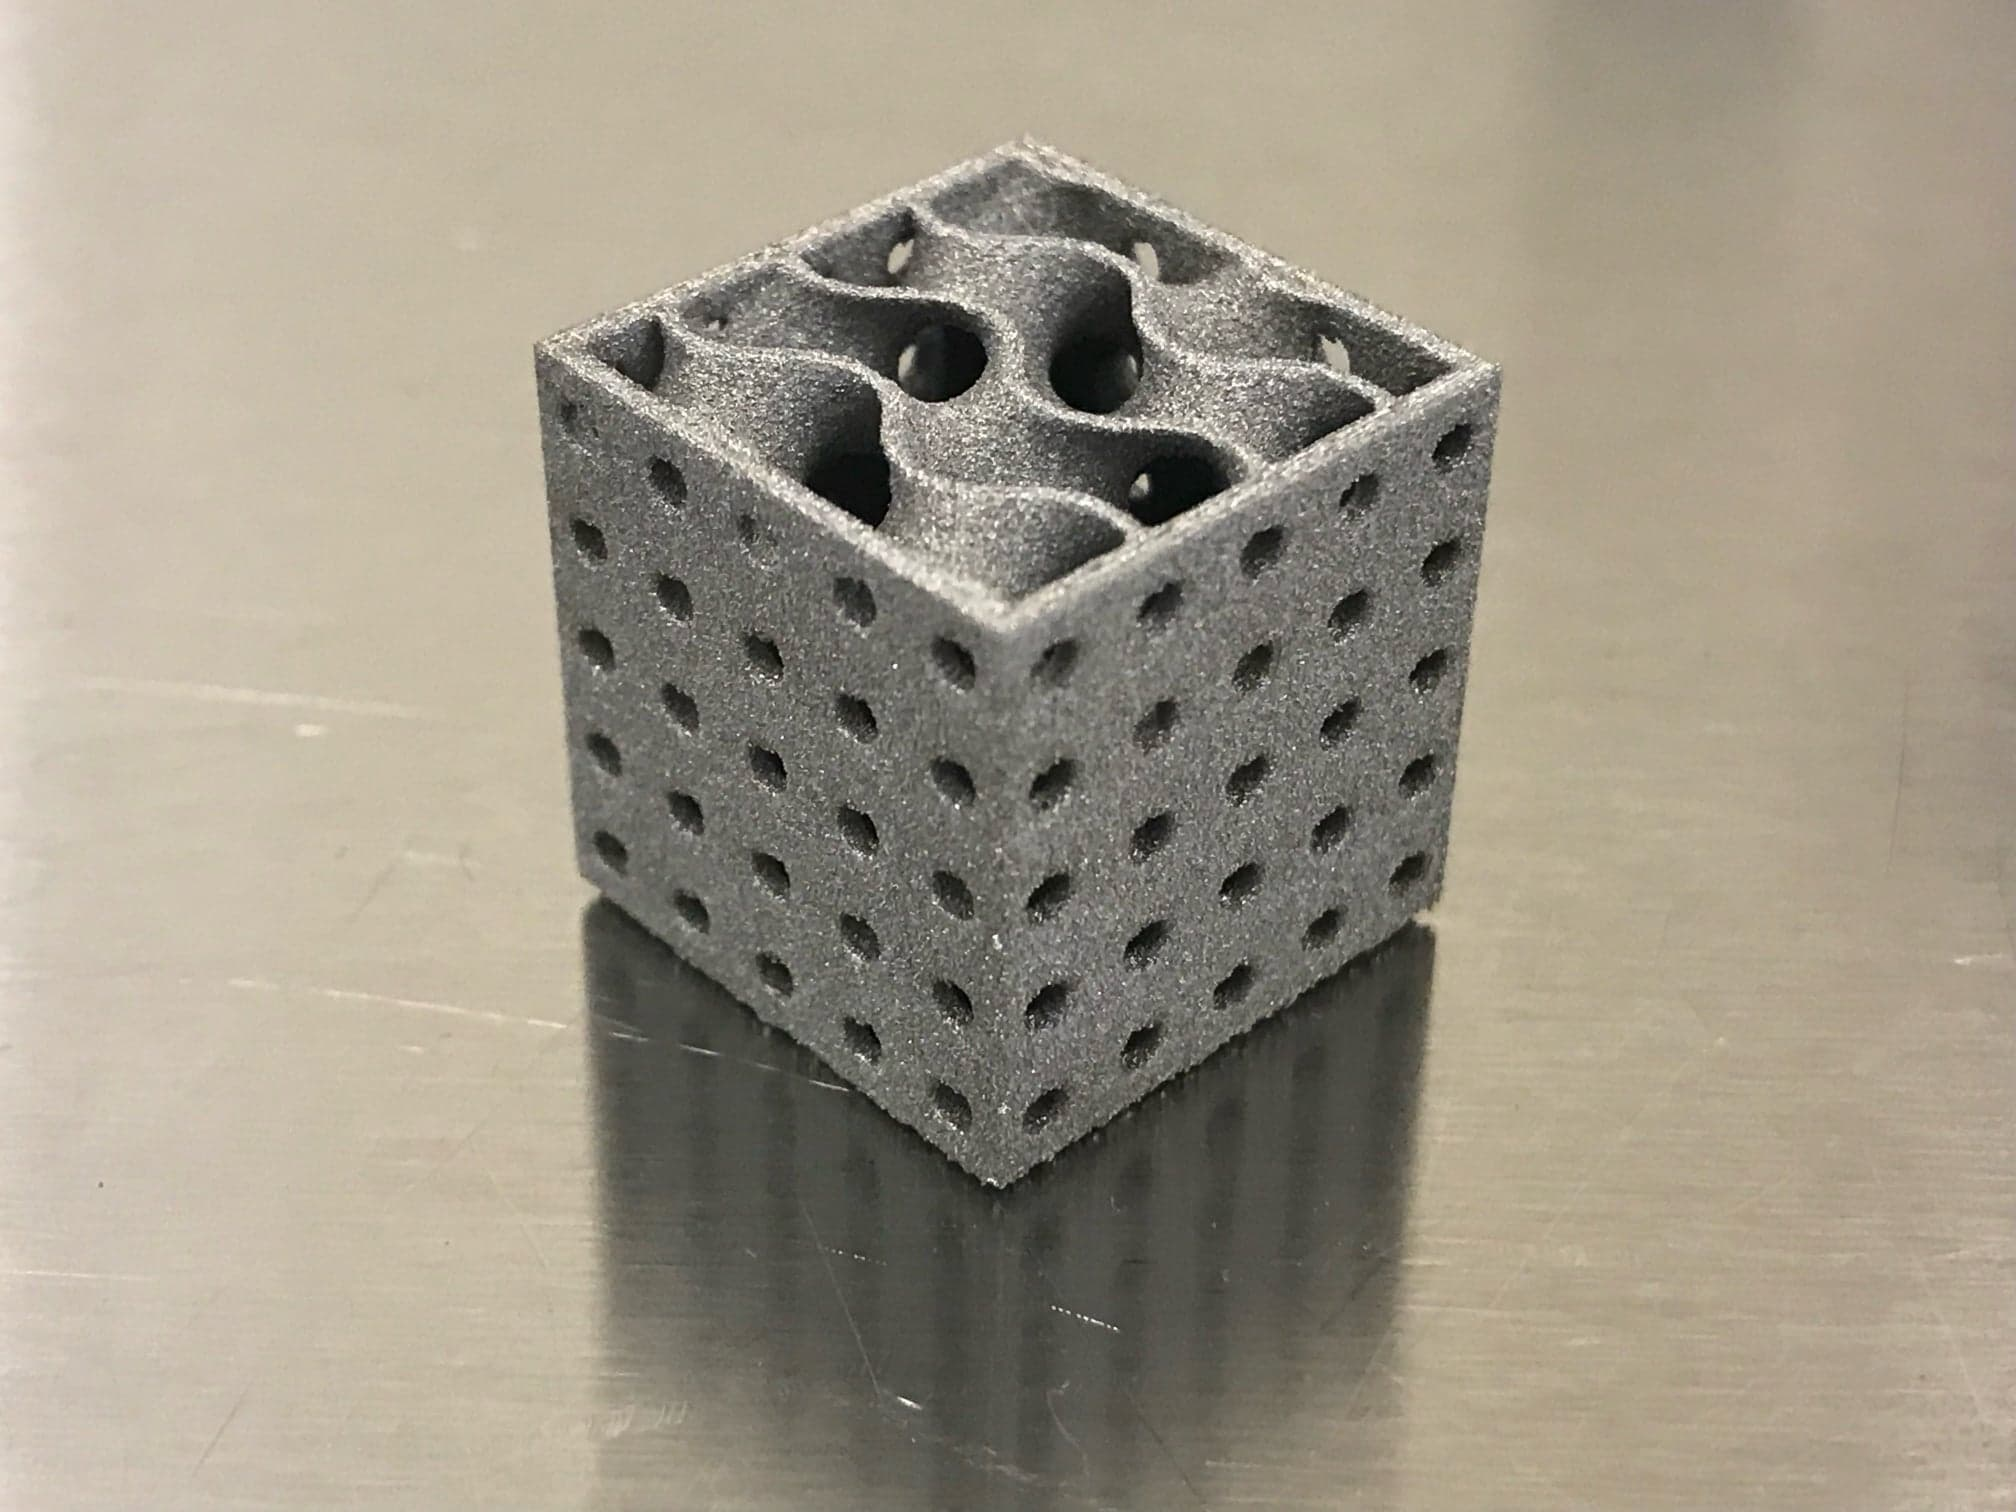
\includegraphics[width=0.3\linewidth]{figures/tungsten-wavy-channels.png}
        \caption{3D printed Tungsten wavy flow channels, reproduced from NASA's Refractory 
        Alloy Additive Manufacturing Build Optimization Project (RAAMBO) 
        \cite{mireles_refractory_2022}.}
    \end{figure}
    \vspace{-0.2cm}
    Wide-spread adoption of 3D printing for reactor parts could reduce 
    fabrication costs, reduce deployment timelines, and improve reactor safety and 
    performance.

    \vspace{0.2cm}
    We require methods, such as \textbf{generative design}, to explore the 
    new design space more efficiently. 
\end{frame}

  \begin{frame}
    \frametitle{Generative Reactor Design Optimization}
    Generative design is an \textbf{iterative design exploration process} \cite{autodesk_autodesk_2020}. 
    \begin{itemize}
        \item Designers provide design goals and constraints to the generative design 
        software
        \item Software explores all the possible permutations of a solution, quickly generating 
        design alternatives
    \end{itemize}
    \vspace{0.2cm}
    The generative design software does not replace the human reactor designer but 
    \textbf{shifts the human designer's focus} away from conjecturing suitable geometries 
    to \textbf{defining the design criteria of optimal designs}. \\

    \textbf{Evolutionary algorithms} can be used to \textbf{drive generative reactor 
    design optimization} to promptly explore the large design space to find global optimal 
    designs. 
  \end{frame}

    \begin{frame}
    \frametitle{Evolutionary Algorithms for Reactor Generative Design}
    \begin{minipage}{0.49\textwidth}
        \textbf{Evolutionary algorithms imitate \\ natural selection} to evolve solutions,  
        and with every generation \textbf{the average population improves}. 

        \vspace{0.3cm}
        Evolutionary Algorithm Benefits 
        \begin{itemize}
            \item Successful at finding multi objective problems' global optimum 
            \item Easily parallelized 
        \end{itemize}
        \end{minipage}
    \begin{minipage}[c]{0.49\textwidth}
        \begin{figure}
            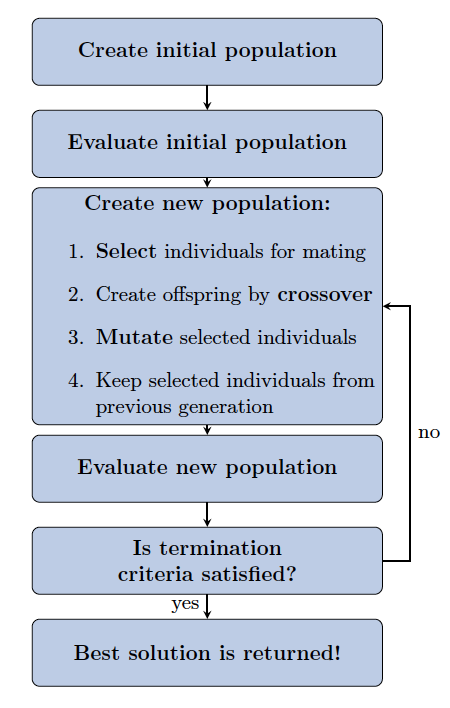
\includegraphics[width=0.7\linewidth]{figures/ea-flow.png} 
            \caption{Evolutionary algorithm flow \cite{renner_genetic_2003}. }
          \end{figure}
    \end{minipage}
    \end{frame}

\subsection{Objectives: AHTR Optimization for Non-Conventional Designs}
\begin{frame}
    \frametitle{Research Objectives: AHTR optimization for non-conventional designs}
    \begin{block}{Technical Gap}
      \begin{itemize}
        \item Optimization tools for generating new reactor designs enabled by
        3D printing do not exist
        \item Few demonstrations of reactor optimization for non-conventional 
        geometries and parameters 
      \end{itemize}
    \end{block}
    \begin{block}{Research Objectives: AHTR optimization for non-conventional designs}
        \begin{itemize}
            \item Develop an open-source tool that enables generative reactor design 
            optimization with evolutionary algorithms 
            \item Demonstrate successful tool application on AHTR optimization for 
            non-conventional reactor geometries and fuel distributions
        \end{itemize}
    \end{block}
  \end{frame}

\subsection{Summary}
\begin{frame}
    \frametitle{Research Objectives Summary}
    \begin{block}{Research Objectives: AHTR Model Development}
        \begin{itemize}
            \item Participate in the OECD-NEA's FHR Benchmark with OpenMC \cite{romano_openmc:_2015}
            \item AHTR temperature model with Moltres \cite{lindsay_moltres_2017}
        \end{itemize}
    \end{block}

    \begin{block}{Research Objectives: AHTR optimization for non-conventional designs}
        \begin{itemize}
            \item Develop an open-source tool that enables generative reactor design 
            optimization with evolutionary algorithms 
            \item Demonstrate successful tool application on AHTR optimization for 
            non-conventional reactor geometries and fuel distributions
        \end{itemize}
    \end{block}
\end{frame}